\documentclass{math}

\usepackage{float}
\usepackage{graphicx}
\usepackage{subcaption}

\title{Introduction to Computer Vision}
\author{Alvin Lin}
\date{August 2018 - December 2018}

\begin{document}

\maketitle

\section*{Segmentation}
Image processing involves an image as input, with the output being another
image. Image analysis outputs measurements from an input image, and image
understanding outputs a high level description from an input image. Humans
tend to identify regions of images in groups, so the goal of segmentation is to
identify groups of pixels or regions that are related and go together
perceptually.

\subsubsection*{Goals of Segmentation}
\begin{itemize}
  \item Obtaining primitives for other tasks
  \item Perceptual organization/recognition
  \item Image manipulation for graphics related tasks.
\end{itemize}
Segmentation can be used to group together similar pixels for efficiency of
further processing (superpixels). It can also separate images into coherent
objects. Oversegmentation and undersegmentation is always an issue here.

\subsection*{High Level Approaches}
Bottom-up segmentation involves grouping tokens with similar features, while
top-down segmentation involves grouping tokens that likely belong to the same
object.
\begin{figure}[H]
    \centering
    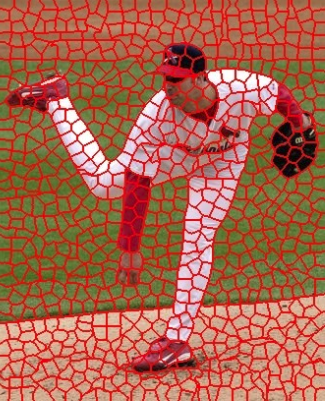
\includegraphics[width=8cm]{assets/segmentation_example1.png}
    \caption{An example of a bottom-up unsupervised approach}
\end{figure}
An alternative approach to this is recognition, or being able to separate the
image into coherent ``objects''. As humans, we can infer a lot of context using
our knowledge to separate out the different elements in an image to identify the
foreground objects. Methods that take the recognition route use a top-down
approach of grouping tokens that likely belong to the same object.

\subsection*{K-means}
Segmentation can be performed through clustering, graph partitioning, and
labeling. With clustering, similar points are grouped together and represented
with a single token. The K-means clustering algorithm can be used to cluster
together similar regions. This will usually find cluster centers that
minimize conditional variance and is simple to implement, however it is prone
to local minima and it is often difficult to choose \( k \). \par
Traditionally, Euclidean distance is used for the K-means clustering algorithm,
but various other metrics can be used.
\begin{itemize}
  \item L1 norm
  \[ d(\vec{x},\vec{y}) = \sum_{i=1}^{n}\|x_i-y_i\| \]
  \item L2 norm
  \[ d(\vec{x},\vec{y}) = \sqrt{\sum_{i=1}^{n}(x_i-y_i)^2} \]
  \item L-infinity
  \[ d(\vec{x},\vec{y}) = max(|x_i-y_i|,\dots,|x_n-y_n|) \]
  \item Mahalanobis distance
  \[ d(\vec{x},\vec{y}) = \sqrt{\sum_{i=1}^{n}\frac{(x_i-y_i)^2}{\sigma_i^2}} \]
  \item Cosine distance
  \[ d(\vec{x},\vec{y}) = \cos(\theta) =
    \frac{\vec{x}\cdot\vec{y}}{\|\vec{x}\|\|\vec{y}\|} \]
\end{itemize}
K-means is usually simple to implement but can be very slow since it is
\( O(kNd) \) for \( N d \)-dimensional points clustered into \( k \) centers.

\subsection*{K-medoids}
Instead of representing a cluster with the mean of its members, we select a
member of the cluster to represent it and minimize cluster dissimilarity. This
is most applicable when the mean is not meaningful. This is much less sensitive
to outliers than k-means. \par
This is a simple and fast alternative to K-means that is easy to implement, but
again depends very heavily on choosing \( k \) correctly. It is rarely used
for pixel segmentation.

\subsection*{Mean Shift Clustering}
The mean shift algorithm seeks modes of the given set of points.
\begin{enumerate}
  \item Choose a kernel and bandwidth.
  \item For each point, center a window on that point and compute the mean of
    the data in the search window. Center the search window at the new mean
    location and repeat until the window convergess.
  \item Assign points that lead to nearby modes to the same cluster.
\end{enumerate}
In addition to storing each pixel's position and color, we can store additional
features such as gradients and texture when performing the mean shift algorithm.
This is typically a very good general purpose segmentation algorithm that is
flexible in the number and shape of regions while being robus to outliers. \par
However, a kernel size must be chosen in advance and it is usually not suitable
for use with high dimensional features. Thus, it is generally used for multiple
segmentations, tracking, clustering, and filtering applications.

\subsection*{Kernel Density Estimation}
Also known as the Parzen-Rosenblatt window method, this is a non-parametric way
to estimate the probability density function of a random variable. Inferences
about a population are made based only on a finite data sample.
\[ \hat{f_h}(x) = \frac{1}{nh}\sum_{i=1}^{n}K\left(\frac{x-x_i}{h}\right) \]
Using the function described above with kernel \( K \) and bandwidth \( h \),
we can generate a relatively smooth curve that very closely models
the distribution of the image.

\subsection*{Segmentation as Graph Partitioning}
If we create a graph with a node for each pixel in an image, we can link nodes
corresponding to adjacent pixels with edges weighted according to the
similarity or affinity of the two nodes. There are a few ways to determine
affinity based on different attributes.
\begin{itemize}
  \item Distance
  \[ d(\vec{x},\vec{y}) = exp\left\{-\frac{(\vec{x}-\vec{y})^t(\vec{x}-\vec{y})}
    {2\sigma_d^2}\right\} \]
  \item Intensity (\( I(x) \) is the intensity of the pixel at \( \vec{x} \))
  \[ d(\vec{x},\vec{y}) =
    exp\left\{-\frac{(I(\vec{x})-I(\vec{y}))^t(I(\vec{x})-I(\vec{y}))}
    {2\sigma_I^2}\right\} \]
  \item Color (\( c(x) \) is the color of the pixel at \( \vec{x} \))
  \[ d(\vec{x},\vec{y}) =
    exp\left\{-\frac{(dist(c(\vec{x}),c(\vec{y})))^2}{2\sigma_c^2}\right\} \]
  \item Texture (\( f(x) \) is a vector of filter outputs at \( \vec{x} \))
  \[ d(\vec{x},\vec{y}) =
    exp\left\{-\frac{(f(\vec{x})-f(\vec{y}))^2(f(\vec{x})-f(\vec{y}))}
    {2\sigma_I^2}\right\} \]
\end{itemize}
After choosing an appropriate feature vector for each pixel and defining an
appropriate distance function, we can break the graph into segments by
deleting links that have low affinity. Similar pixels should be in the same
segments while dissimilar pixels should be in different segments. A graph cut
allows us to make a good segmentation by removing enough edges to fully
disconnect discrete segments. \par
One method of doing this is by finding the minimum cut of the graph (for which
fast algorithms already exist). This tends to cut off small and isolated
segments however, so we can fix this by using a normalized cut where we
normalize the cut by the weight of all the edges incident to the segment. We
compute a new normalized cut cost
\[ cost(A,B) = \frac{w(A,B)}{w(A,V)}+\frac{w(A,B)}{W(B,V)} \]
where \( w(A,B) \) is the sum of the weights of all edges between \( A \) and
\( B \). Finding the globally optimal cut is an NP-complete problem, but a
relaxed version can be solved using a generalized eigenvalue problem. This is
a generic framework that can be used with many different features and affinity
formulations but has a high storage requirement and time complexity due to
solving a generalized eigenvalue problem of size \( n\times n \) where \( n \)
is the number of pixels.


\begin{center}
  You can find all my notes at \url{http://omgimanerd.tech/notes}. If you have
  any questions, comments, or concerns, please contact me at
  alvin@omgimanerd.tech
\end{center}

\end{document}
